\documentclass{article}
\usepackage{amsmath}
\usepackage{pgfplots}
\pgfplotsset{compat=1.16}

\begin{document}

\begin{figure}[h]
    \centering
    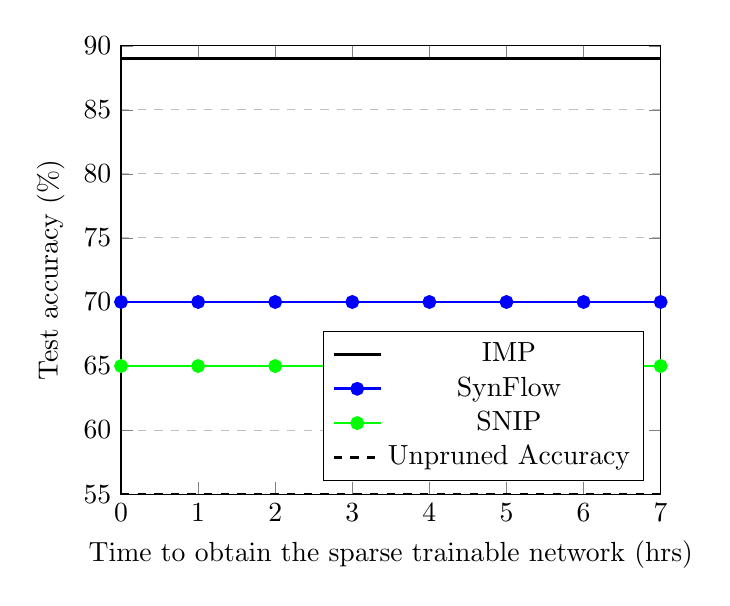
\begin{tikzpicture}
        \begin{axis}[
            title={},
            xlabel={Time to obtain the sparse trainable network (hrs)},
            ylabel={Test accuracy (\%)},
            xmin=0, xmax=7,
            ymin=55, ymax=90,
            xtick={0,1,2,3,4,5,6,7},
            ytick={55,60,65,70,75,80,85,90},
            legend pos=south east,
            ymajorgrids=true,
            grid style=dashed,
        ]
        \addplot[
            color=black,
            mark=none,
            line width=1pt,
        ]
        coordinates {
            (0,89) (1,89) (2,89) (3,89) (4,89) (5,89) (6,89) (7,89)
        };
        \addlegendentry{IMP}

        \addplot[
            color=blue,
            mark=*,
            line width=1pt,
        ]
        coordinates {
            (0,70) (1,70) (2,70) (3,70) (4,70) (5,70) (6,70) (7,70)
        };
        \addlegendentry{SynFlow}

        \addplot[
            color=green,
            mark=*,
            line width=1pt,
        ]
        coordinates {
            (0,65) (1,65) (2,65) (3,65) (4,65) (5,65) (6,65) (7,65)
        };
        \addlegendentry{SNIP}

        \addplot[
            color=black,
            mark=none,
            line width=1pt,
            dashed,
        ]
        coordinates {
            (0,55) (1,55) (2,55) (3,55) (4,55) (5,55) (6,55) (7,55)
        };
        \addlegendentry{Unpruned Accuracy}
        \end{axis}
    \end{tikzpicture}
    \caption{Comparing test accuracy of sparse networks derived using early pruning methods for AlexNet with 99.3\% parameters removed and trained on the CIFAR-10 dataset. The x-axis shows the time taken to obtain the sparse trainable network.}
\end{figure}

\end{document}